\section{Сеточная функция} \label{grid}
Для аппроксимации системы дифференциальных уравнений (\ref{eq1:system}) разностным методом для начала введем пространственно - временную сетку на плоскости $x = (x_{1},x_{2})$ с координатами $x^{i}_{1} = i \cdot h_{1},\; x^{j}_{2} = j \cdot h_{2} , \; t^{k} = k \cdot \tau $, где $h_{1},\; h_{2}$ -- шаги по пространству, $\tau$ - шаг по времени; $i = \overline{0,N}, j = \overline{0,M}$ и $k = \overline{0,T}$. Таким образом, вся расчетная область покрывается сеткой (рис. \ref{fig:grid}).

\begin{figure}[ht]
    \centering
    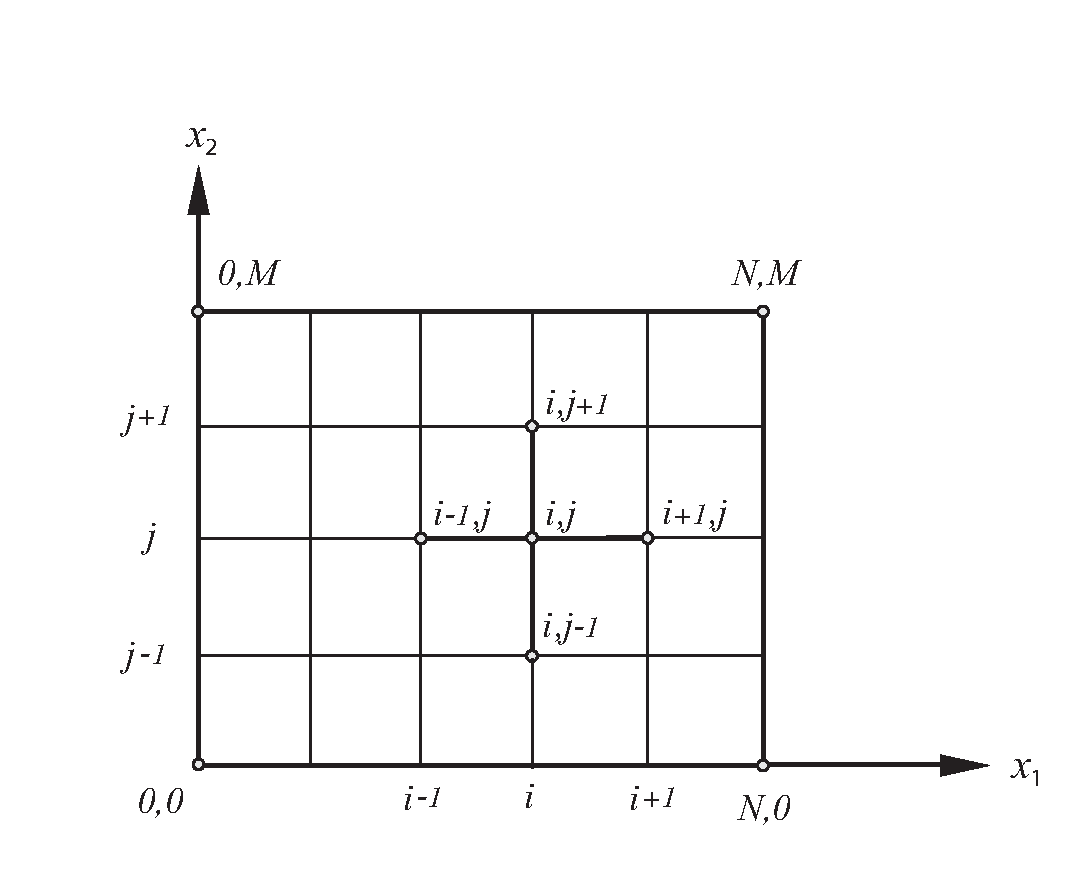
\includegraphics[scale = 0.5]{grid}
    \captionsetup{justification=centering,margin=2cm}
    \caption{Разностная сетка области решения}
    \label{fig:grid}
\end{figure}

 Узлы которые попали внутрь $\Omega$, назовем \textit{внутренними}, а их совокупность обозначим $\omega_{h}$. Точки пересечения прямых $x^{i}_{1} = i \cdot h_{1}$ и $x^{j}_{2} = j \cdot h_{2}$ с границей $\Gamma$ назовем \textit{граничными}, а множество всех граничных узлов обозначим $\gamma_{h}$.
 
 И так, область изменения аргумента $x = (x_{1},x_{2})$ заменяется сеткой  $ \overline{\omega_{h}} = \omega_{h} + \gamma_{h}$, то есть конечным множеством точек $x^{i}_{1}, x^{j}_{2}$, принадлежащих $\overline{\Omega} = \Omega + \Gamma$. И вместо функции $u(x_{1},x_{2},t)$ непрерывного аргумента $x \in \overline{\Omega} $ будем рассматривать сеточные функции $y(x^{i}_{1},x^{j}_{2},t^{k})$ \cite[Самарский][67]{Samarskiy1977}.